%%% New implementation section

\section{Monitor Implementation and Evaluation}
\label{sec:implementation}

%% paragraph 1 -- goals
To evaluate the feasibility of our monitoring algorithm for safety-critical
real-time systems we have built a real-time CAN monitor on an ARM Cortex-M4
development board. This allowed us to explore the necessary optimizations and
features required to perform real-time checking of realistic safety policies.

%% paragraph 2 -- what we built

%% Embedded restrictions
\noindent\textbf{Challenges. }
Software for safety-critical embedded systems typically contains more strict
design and programming model constraints than less critical software. Two
important and common constraints for these systems are avoiding recursion  and
 dynamic memory allocation.
% dynamic memory alloc
% Common safety-critical coding guidelines discourage or prohibit dynamic memory
% allocation to avoid memory leaks.
As \planguage is bounded, we avoid dynamic allocation
in our \monitor implementation by statically allocating space for the maximum
number of entries for our history structures and other temporary data structures.
% recursion
% Recursion is also usually prohibited because it can be difficult to guarantee a
% maximum stack depth when using recursion.
Although \monitor is defined recursively,
we  implement \monitor using a traditional iterative traversal
of the specification formulas instead.

\noindent\textbf{Discussion. }
Passive monitoring of running systems requires attention to timing issues with regards to system state sampling.
%
The monitor possesses a copy of the target system state and
when a new CAN message from the system is seen it updates this
system state based on the incoming message. In short, the monitor periodically
takes a snapshot of this constantly updated state and uses that snapshot
as the trace state which is monitored.
%
Thus, the actual monitored state (\ie, the trace) is a discrete sampling of the monitor's constantly updated system state. 
The monitor's period must be fast enough that any changes in system state which are relevant to the specification are seen in the sampled trace.
To ensure this, the monitor's period should be twice as fast as the shortest CAN message period, which ensures the monitored trace contains every value seen on the CAN bus.
If the monitor period is not fast enough, multiple CAN messages announcing the same system value may end up in the same trace state, which can cause those value changes to not be seen in the trace.
For example, if the monitor is sampling at $2ms$, and three messages announcing the value of property $X$ are received at times $0ms$, $1ms$, and $1.5ms$, only the value announced at $1.5ms$ will be seen in the trace. To avoid this, the monitor would need to run faster than the messages interarrival rate (at least $0.5ms$ in this case).

Along with requiring the monitor to sample its trace state fast enough to see all the relevant state changes, the specification time bounds must be a multiple of the monitoring period.
This ensures that each time step in the formula is evaluated on the updated information.
A simple way of understanding this is to use monitor steps as the temporal bounds instead of explicit time bounds.
For example, if the monitor is running at  2ms intervals, we can use $\henceforth_{[0,50]} p$ as an equivalent to
$\henceforth_{[0,100ms]} p$.
As the monitored trace state is only updated at 2ms, the state is unchanged
from 0-2ms, and then again from 2-4ms, etc.
If a bound is not a multiple of the monitor's interval, then formulas with
different bounds can look indistinguishable,
\eg, $\henceforth_{[0,5ms]} p$ is equivalent to $\henceforth_{[1ms,4ms]} p$
for a $2ms$ monitor.
% Since this is unintiutive, using steps or period-multiple
% bounds is best.
%
To summarize, using a monitoring period at least twice as fast as the shortest
CAN message period (\ie, shortest time between a CAN message retransmission)
and only using temporal bound values that are multiples of this period provides intuitive monitoring results.


\noindent\textbf{Hybrid Algorithm (\ha).}
%Our eager monitoring algorithm attempts to evaluate specification rules as soon as possible, but this requires checking trace properties which may not be fully reducible given the current trace. These unfinished formula reductions require extra computation time, and in practice the majority of the policy reductions performed by \monitor will be these eager reductions which may not fully reduce.
The eager monitoring algorithm attempts to evaluate specification rules as soon as possible
which requires checking properties which may not be fully reducible given the current trace.
While early detection of violations can be useful, continuously attempting to check
partially reduced residues which need future information to evaluate requires extra computation.
%While early detection of violations can be useful, the costs of re-reducing partially reduced residues can become large given the right formula and trace.
In some cases, the worst-case execution time to eagerly check a property (or set of properties)
over a trace may be longer than the monitor's period.
In this case the eager algorithm cannot guarantee prompt monitoring since some
residues will be left unchecked. This is unacceptable for
safety-critical system monitoring, as without a promptness guarantee the results cannot be fully trusted. 
%Even if this worst-case situation does not occur, for monitoring safety-critical systems the monitor must be able to guarantee completion.
%there are situations where eagerly checking an entire target specification may require more computation than is available from the monitor in a given period.
%
To enable the benefits of eager checking while avoiding the risks of losing
real-time correctness, we can use a hybrid approach (called \ha) which first performs non-eager
(conservative) checking and then uses any spare time left in the monitoring period to
perform as much eager checking as possible.
\ha preserves the monitor's promptness guarantee (all violations will be
detected within their delay $\wdelay$) even if the \monitor cannot finish eager
checking the specification.
\ha preserves promptness while providing a chance to eagerly detect specification violations.
\ha is functionally equivalent to \monitor when it finishes
execution before the monitoring period whereas \ha is
% when it is able to keep up with the trace, and
equivalent to the conservative algorithm when there is no spare execution time to perform eager checks.

Figure \ref{fig:hybrid_comp} shows the detection latency for the hybrid algorithm checking  the property $(\pred{CruiseActive} \wedge \pred{brakePressed} \rightarrow \henceforth_{[250ms, 1s]} (\neg \pred{CruiseActive})$ over an artificial log using different monitor periods. 
With a $1ms$ period the monitor is able to eagerly detect every violation as eagerly as soon as possible (\ie, when the first false inside the always occurs). 
The $8.2us$ period is able to detect some violations early, but it does not detect them as early as possible. 
The $1us$ period is too fast and the hybrid check only provides conservative checking, identifying the violations at the promptness limit of $1s$.

\begin{figure}[t]
\centering
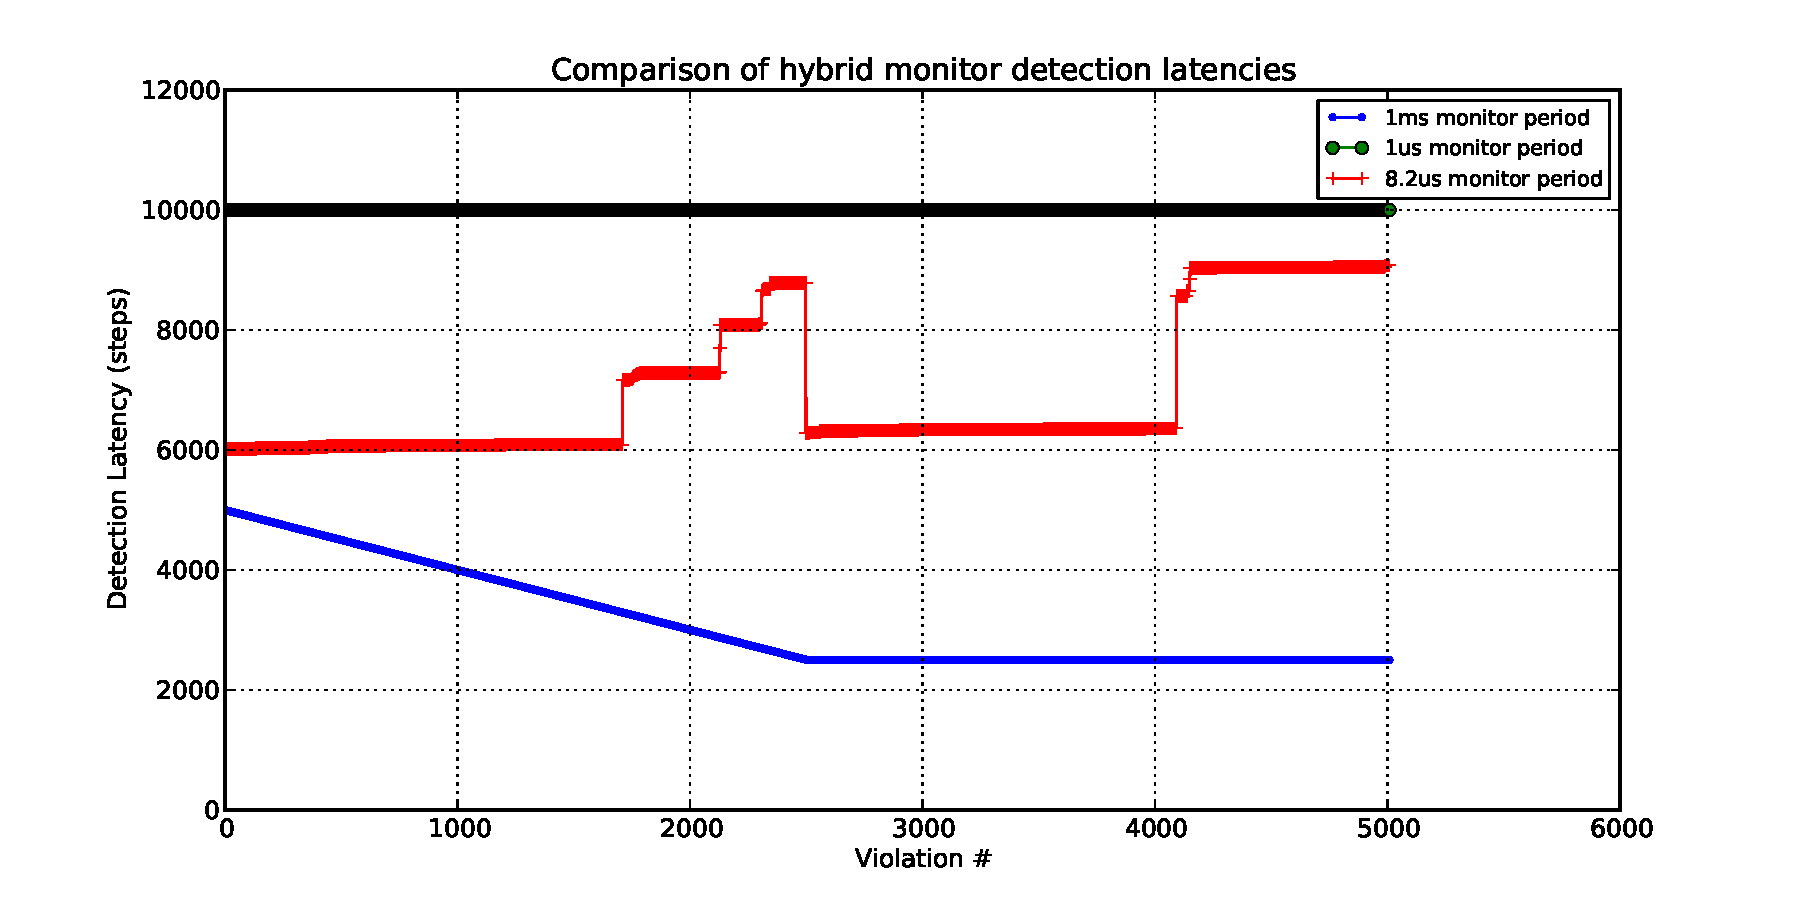
\includegraphics[width=4in]{img/hybrid_comp}
\caption{Detection latencies with different hybrid monitor periods\label{fig:hybrid_comp}}
\end{figure}
%we have implemented a hybrid eager monitoring algorithm which performs non-eager (conservative) checking first and uses any spare time to eagerly check the remaining monitor residues.
%
%Conservative \monitor monitoring is performed by only checking residues which are older than their formula delay, which guarantees that these residue will be reduced at their first evaluation. For a periodic monitor this only requires updating the history structures and checking a single residue for each policy.
%
%This conservative check can be done quickly at each period, leaving any extra time until the next period for eager checking. This provides a conservative monitoring guarantee (\ie, the specification is checked within a known promptness delay) while also allowing the monitor to eagerly check as much of the specification as possible.
%
%As long as we know that the worst case execution time for message handing, incrementing the structures, and a single residue check is short enough to finish within a monitor period then we are guaranteed at least a conservatively correct and prompt output.
%
% \begin{figure}[tbp]
% \centering
% 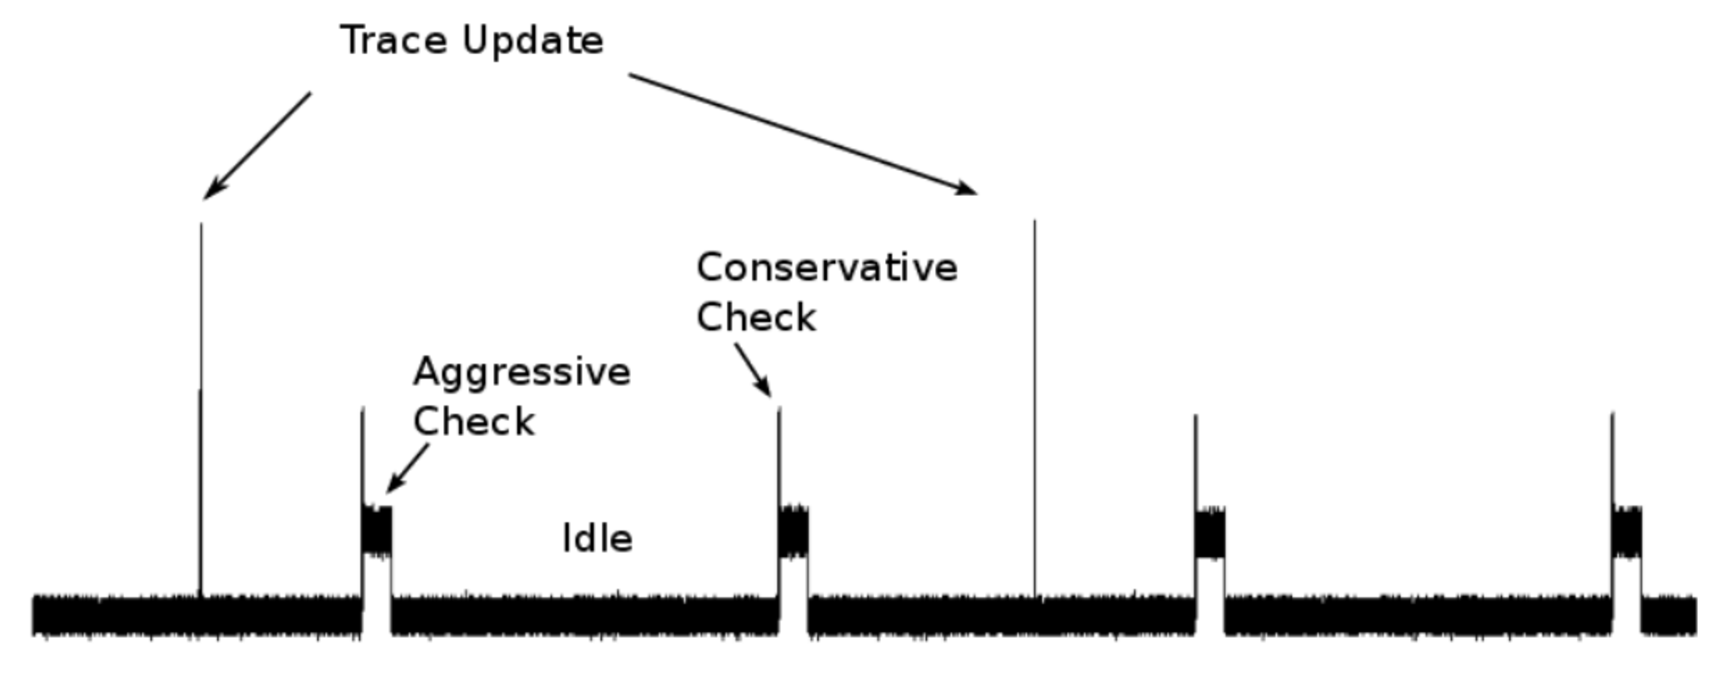
\includegraphics[width=3.7in]{img/scope_annotated_crop}
% \caption{Oscilloscope capture of embedded monitor task execution \label{fig:arch:oscope}}
% \end{figure}
%
We have also implemented \ha in our embedded board.
\ha updates the history structures (shared between
the conservative and eager checking) and
performs a conservative check once every monitoring period.
It then uses the idle time between periods to perform eager
checking of any remaining unchecked specification properties.
The eager checking gets interrupted  by the next period
when the extra time runs out.
% replacing oscope figure info with hybrid eval description
%@TODO update this
%A quick evaluation of the hybrid monitor against offline logs demonstrates the usefulness and functionality of the hybrid approach. Figure \ref{fig:hyb_eval} shows the detection latency of specification violations for a specification with moderate temporal size.


%% This is all oscope figure stuff, replaced with hybrid analysis
%
% Figure \ref{fig:arch:oscope} shows the execution of the embedded monitor
% instrumented to output the currently executing task to an oscilloscope.
%The residue checks run twice per trace update due to the monitor configuration used during the test, but this is not required for correct monitoring.
%This task output was captured while monitoring the specification used in the case study (see Section \ref{sec:case_study}) plus another 200 time-step \emph{eventually} rule which was never satisfied.
%(guaranteeing an extra 200 eager residue checks every period).
%The rule never being satisfied means that the monitor performed an eager check of all 200 residues for this rule at every step (i.e., since they were never satisfied, they could never be reduced early).
%Even with this excess computation there was still a large portion of extra idle time -- 23ms of the 25ms monitoring loop was spent idle.
%This shows the eager checking finished reasonably quickly and the monitor could handle much longer formula durations or more complex formulas before the execution time becomes bad enough to require the hybrid algorithm for correctness guarantees.

\subsection{Case Study}
\label{sec:case_study}
This section reports our case study performing real-time monitoring of a CAN network for realistic safety properties.
For this case study we have obtained CAN network logs from a series of robustness tests on the ARV which we have replayed on a test CAN bus for the monitor to check.
This setup %, shown in Figure \ref{fig:replaySchem},
helps us show the feasibility of performing external bus monitoring on this class of system with real safety specifications.

%% removing, takes space and not that important
%\begin{figure}
%\centering
%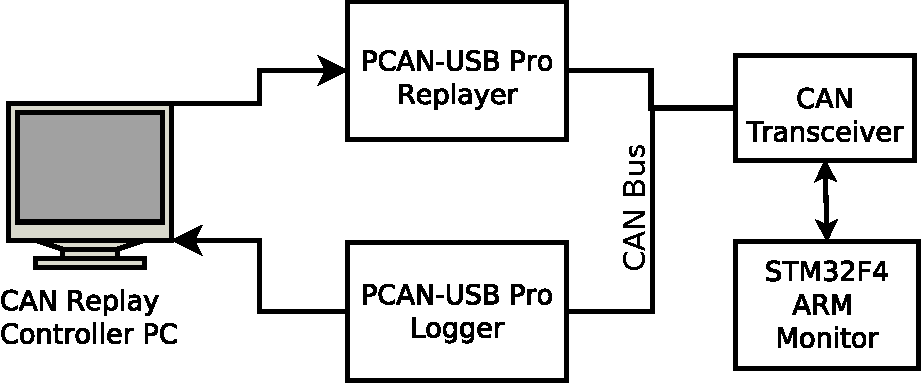
\includegraphics[width=3in]{img/replay_arch}
%\caption{CAN replay network setup \label{fig:replaySchem}}
%\end{figure}

%% paragraph 3 -- description of experiment
%%% some of this is in para1, we should go over: specification, logs, etc
The logs contain both normal system operation as well as some operation under network-based robustness testing. During robustness testing, the testing framework can intercept targeted network messages on the bus and inject its own testing values. % could cite astaa here
A PC was connected to a PCAN-USB Pro \cite{PCAN-USBPro} device which provides a USB interface to two CAN connections. One CAN channel was used to replay the logs, while the other was used as a bus logger for analysis purposes.

%% paragraph 4 -- specification
Requirements documentation for this system was available, so we were able to build a monitoring specification based on actual system requirements.
The specification evaluated in the embedded monitor on the test logs are shown in Table \ref{tab:monspec}. This specification was derived from the system requirements based on the observable system state available in the testing logs.
% acknowledge that case study looks simple -- but there are reasons for that
We note that the safety specification is simple and does not fully excercise the monitor's constraints. Safety specifications derived from common system safety analysis would likely have a larger number of rules with similar complexities.
Monitoring additional rules scales well as each rule adds at worst it's own checking time independent of the other rules and
also because independent rules can be split up across multiple monitors.
%
% don't need hybrid here
Since this specification is small, does not have long duration future-time formulas,
and the monitor period is relatively slow ($25ms$) \ha and \monitor functions equivalently
for the case study -- \monitor can always finish within the monitoring period in the worst case.
We were able to eagerly monitor this specification plus an additional 200 residues in under $2ms$.
If the specification properties required a faster trace resolution we would run into
worst-case speed problems for \monitor and would require to use \ha.
%
We use the \ha for the study since it acts the same as \monitor when there is excess monitoring time.
Using \ha helps us avoid worrying about the execution time.
As long as the monitor can finish the conservative checks and
history structure update within the period the monitor will be prompt.



\begin{table}[t]
\centering
%\begin{tabular}{|p{3in}|l|}
\footnotesize
\begin{tabular}{|c|p{4.3in}|}
\hline \multirow{2}{*}{Rule \#} & Informal Rule \\ & MTL \\
\hline \multirow{2}{*}{0} & A feature heartbeat will be sent within every 500ms \\
& $\pred{HeartbeatOn} \rightarrow \LTLdiamond_{[0,500ms]} \pred{HeartBeat}$ \\
\hline \multirow{2}{*}{1} & The interface component heartbeat counter is correct \\
& $\pred{HeartbeatOn} \rightarrow \pred{HeartbeatCounterOk}$ \\
\hline \multirow{2}{*}{2} & The vehicle shall not transition from manual mode to autonomous mode \\
&  $\neg ((\LTLcircleminus_{[0,25ms]} \pred{IntManualState}) \wedge \pred{IntAutoStat})$\\
\hline \multirow{2}{*}{3} & The vehicle controller shall not command a transition from manual mode to autonomous mode \\
& $\neg ((\LTLcircleminus_{[0,25ms]} \pred{VehManualModeCmd}) \wedge \pred{VehAutoModeCmd})$\\
\hline \multirow{2}{*}{4} & The vehicle shall not transition from system off mode to autonomous mode \\
&  $\neg ((\LTLcircleminus_{[0,25ms]} \pred{IntSDState}) \wedge \pred{IntAutoStat})$\\
\hline \multirow{2}{*}{5} & The vehicle controller shall not command a transition from system off mode to autonomous mode \\
& $\neg ((\LTLcircleminus_{[0,25ms]} \pred{VehSDModeCmd}) \wedge \pred{VehAutoModeCmd})$\\
% warn was at 200ms
\hline
\end{tabular}
\caption{Case study monitoring specification \label{tab:monspec}}
\end{table}

$\pred{HeartBeatOn}$ is a guard which is true when once the target component has started in the logs (to avoid false-positive missing heartbeats during system startup).
The system's heartbeat message contains a single heartbeat status bit which we checked directly in Rule \#0 to ensure the component is still running (essentially a watchdog message).
The heartbeat message also has a rolling counter field.
We use the \sfmap to ensure that this counter is incrementing correctly and output this check as the $\pred{HeartbeakOk}$ proposition which is monitored in Rule \#1.
%Rule \#0 is a heartbeat detection which ensures that the interface component is still running (essentially a watchdog message).  Rule \#1 is a second component of this check.
We also checked for illegal state transitions. Rules \#2 through \#5 check both for illegal transition commands from the vehicle controller and actual illegal state transitions in the interface component.

%% move hybrid algorithm explanation here maybe?

\subsection{Monitoring Results}
Monitoring the test logs with the above specification resulted in identifying two real violations as well as some false positive violation detections caused by the testing infrastructure.
%
% covering all three possible violation types. One was a false positive
Three different types of heartbeat violations were identified after inspecting the monitor results, with one being a false positive.
%some actual violations and some false-positives caused by the testing infrastructure.
We also identified infrastructure-caused false-positive violations of the transition rules.

\begin{figure}[t]
		\centering
		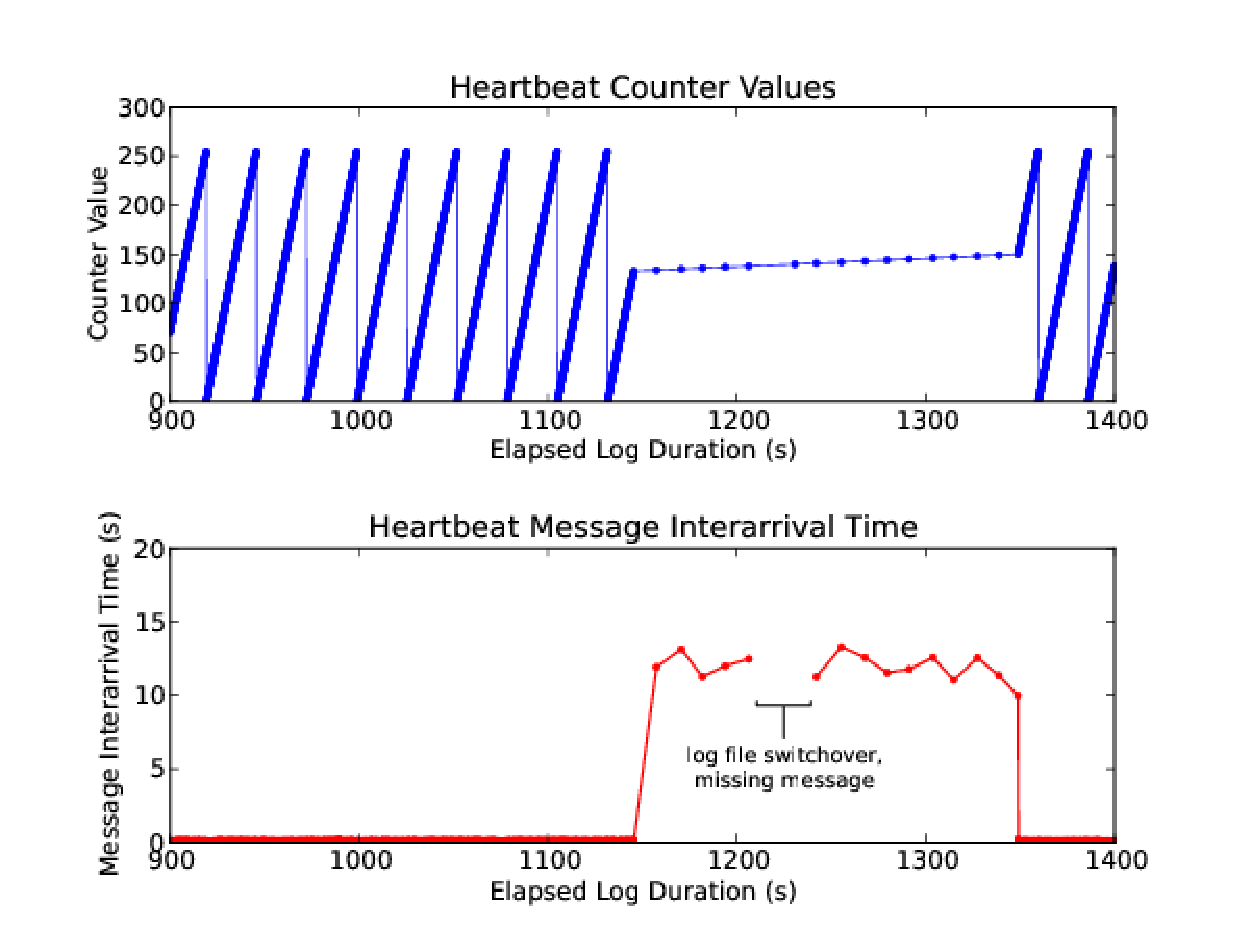
\includegraphics[width=4.0in]{img/hb1}
		\caption{Heartbeat counter values over time}
		\label{fig:hb_arrival}
\end{figure}

\textit{Specification violations.}
% missing hb message
The first violation is a late heartbeat message. In one of the robustness testing logs the heartbeat message was not sent on time, which is clearly a heartbeat violation. Figure \ref{fig:hb_arrival} shows the heartbeat counter values and the inter-arrival time of the heartbeat messages over time for this violation. We can see here that the heartbeat counter did in fact increment in a valid way, just too slowly.
% bad status
The second violation is on-time heartbeat status message but the heartbeat status field is 0.
We do not know from the available documentation whether a bad status in an on-time message with a good counter is valid or not. So without more information we cannot tell whether these violations are false positives or not. This is worthy of further investigation.


\begin{figure}[t]
\centering
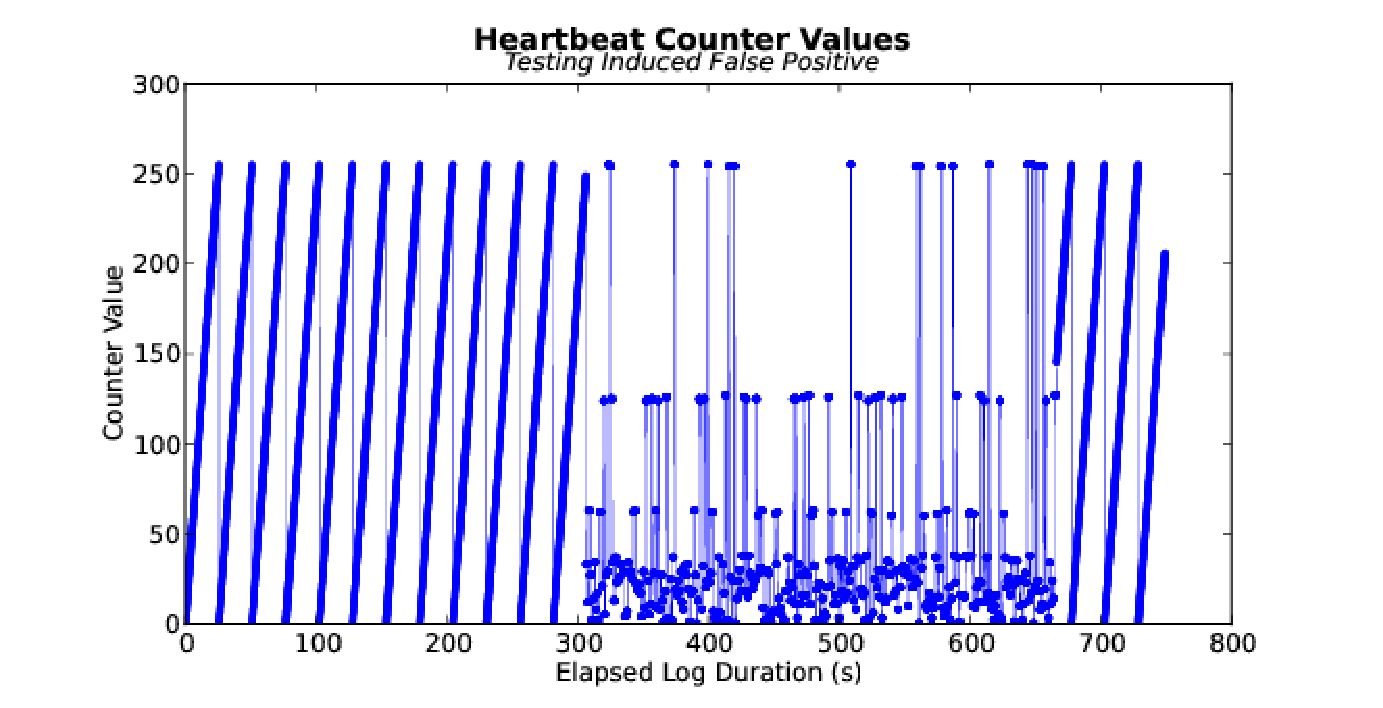
\includegraphics[width=4.0in]{img/hb2}
\caption{Bad heartbeat counter values \label{fig:hb_badcounter}}
\end{figure}

\textit{False-positive violations.}
% bad counter
The last type of heartbeat violation is a bad counter.
A good rolling counter should increment by one every message up to its maximum (255 in this case) before wrapping back to zero.
%We have defined a good counter as one which increments by one every message up to its maximum (255 in this case) before wrapping back to zero.
Every consecutive heartbeat status message must have an incremented heartbeat counter or a violation will be triggered. Figure \ref{fig:hb_badcounter} shows the counter value history for one of the traces with a heartbeat violation caused by a bad counter value.
%
%@EDIT describe robustness testing, define these false positives like the talk?
Further inspection of this violation showed that the bad counter values were sent by the testing framework rather than the actual system. In this case, the network traffic the monitor is seeing is not real system state
instead are observing
% but actually it is
messages that are being injected by the testing framework.
This is not a real violation (since the violating state is not the actual system state),
and so we consider this a false positive violation.



The monitor also reported violations of the legal transition rules, but these, similar to the heartbeat counter violation, also turned out to be false positives triggered by message injections by the robustness testing harness. Since the monitor checks network state, if we perform testing that directly affects the values seen on the network (such as injection/interception of network messages) we may detect violations which are created by the testing framework rather than the system.
Information about the test configurations can be used to filter out these types of false positives which arise from test-controlled state.
This type of filtering can be automated if the test information can be input to the monitor, either directly on the network (e.g., adding a message value to injected messages) or through a side-channel (i.e., building a testing-aware monitor).
